\documentclass[12pt]{article}
\usepackage[margin=1in]{geometry}
\usepackage{hyperref}
\usepackage{booktabs}
\usepackage{tikz}
\usetikzlibrary{arrows.meta,positioning}

\title{Healthcare Scam / Phishing Detector}
\author{Anmol Rathod}
\date{\today}

\begin{document}
\maketitle

\begin{abstract}
This project presents a lightweight machine learning system for detecting healthcare-related scam and phishing messages. The system combines public SMS spam data with healthcare-focused examples, applies text cleaning and TF-IDF feature engineering, compares multiple classical classifiers, and deploys the selected model through a Streamlit interface.
\end{abstract}

\section{Introduction}
Healthcare communication increasingly occurs through SMS, email, and patient portals. Attackers exploit this trust with fake insurance notices, Medicare card warnings, billing threats, and credential theft requests.

\section{Problem Statement}
The objective is to classify a message as legitimate or scam/phishing while minimizing false negatives, because missed scams can lead to identity theft, financial loss, and privacy harm.

\section{Motivation}
Healthcare scams target vulnerable users and often imitate official organizations. A practical screening tool can help users pause and verify suspicious messages before responding.

\section{Literature Review}
Classical NLP models such as Logistic Regression, Naive Bayes, and Linear SVM remain strong baselines for short-text spam detection. TF-IDF features are efficient, interpretable, and suitable for laptops without GPU requirements.

\section{Dataset}
The project uses the UCI SMS Spam Collection as a public baseline and a curated healthcare seed dataset for domain-specific examples. Labels are mapped into two classes: legitimate and scam.

\section{Data Cleaning}
Preprocessing normalizes whitespace, removes duplicate messages, validates required columns, and maps compatible labels such as ham, spam, phishing, and smishing into the project label space.

\section{Feature Engineering}
Messages are vectorized using TF-IDF with unigram and bigram features. English stop words are removed to emphasize discriminative terms.

\section{ML Pipeline}
The pipeline performs train/test splitting, stratified cross-validation, hyperparameter tuning, model comparison, final model selection, and persistence with joblib.

\section{Model Comparison}
The compared models are Logistic Regression, Multinomial Naive Bayes, Linear SVM, and Random Forest. Selection prioritizes scam recall, then scam F1-score, then accuracy.

\section{Results}
Results are generated reproducibly in \texttt{models/metrics.json}. The evaluation includes accuracy, precision, recall, F1-score, ROC-AUC when applicable, and confusion matrix output.

\section{Architecture Diagram}
\begin{center}
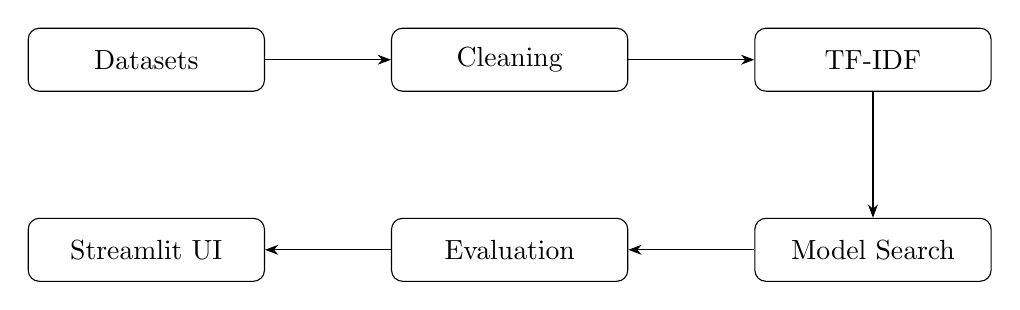
\begin{tikzpicture}[node distance=1.6cm, every node/.style={draw, rounded corners, align=center, minimum width=3cm, minimum height=0.8cm}, >={Stealth}]
\node (data) {Datasets};
\node[right=of data] (clean) {Cleaning};
\node[right=of clean] (tfidf) {TF-IDF};
\node[below=of tfidf] (models) {Model Search};
\node[left=of models] (eval) {Evaluation};
\node[left=of eval] (app) {Streamlit UI};
\draw[->] (data) -- (clean);
\draw[->] (clean) -- (tfidf);
\draw[->] (tfidf) -- (models);
\draw[->] (models) -- (eval);
\draw[->] (eval) -- (app);
\end{tikzpicture}
\end{center}

\section{UI Workflow}
The user pastes a message, clicks Analyze, receives a label, confidence score, suspicious keyword highlights, explanation, and prediction history.

\section{Limitations}
The included healthcare examples are small and should be expanded with licensed real-world healthcare phishing data before production use. Attackers also change language over time, requiring periodic retraining.

\section{Future Scope}
Future improvements include larger healthcare-specific datasets, threshold tuning, explainability methods such as LIME or SHAP, multilingual support, and API deployment.

\section{Conclusion}
The project demonstrates a complete, explainable, and lightweight healthcare scam detection workflow suitable for internship and portfolio presentation.

\section{References}
\begin{itemize}
\item UCI Machine Learning Repository, SMS Spam Collection.
\item Almeida, T. A., Hidalgo, J. M. G., and Yamakami, A. Contributions to SMS spam filtering research.
\item Nazario Phishing Corpus.
\end{itemize}

\end{document}
